\documentclass[onecolumn, letter, 11pt]{article}

\usepackage{fourier}
\usepackage[utf8]{inputenc}
\usepackage[sumlimits]{amsmath}
\usepackage{graphicx}
\usepackage[spanish]{babel}
\usepackage{amsfonts}
\usepackage{amssymb}
\usepackage{amsthm}
\usepackage{geometry}

\geometry{left=2.5cm,right=2.5cm,top=2.5cm,bottom=2.5cm}


\title{Examen rápido No. 9}
\author{Inteligencia Artificial, curso 2018-1\\ \textsc{Julio Waissman Vilanova}}
\date{}


\begin{document}

\maketitle

\section{Inferencia aproximada}

De acuerdo a la siguiente red bayesiana, realiza lo que se pide

\begin{center}
  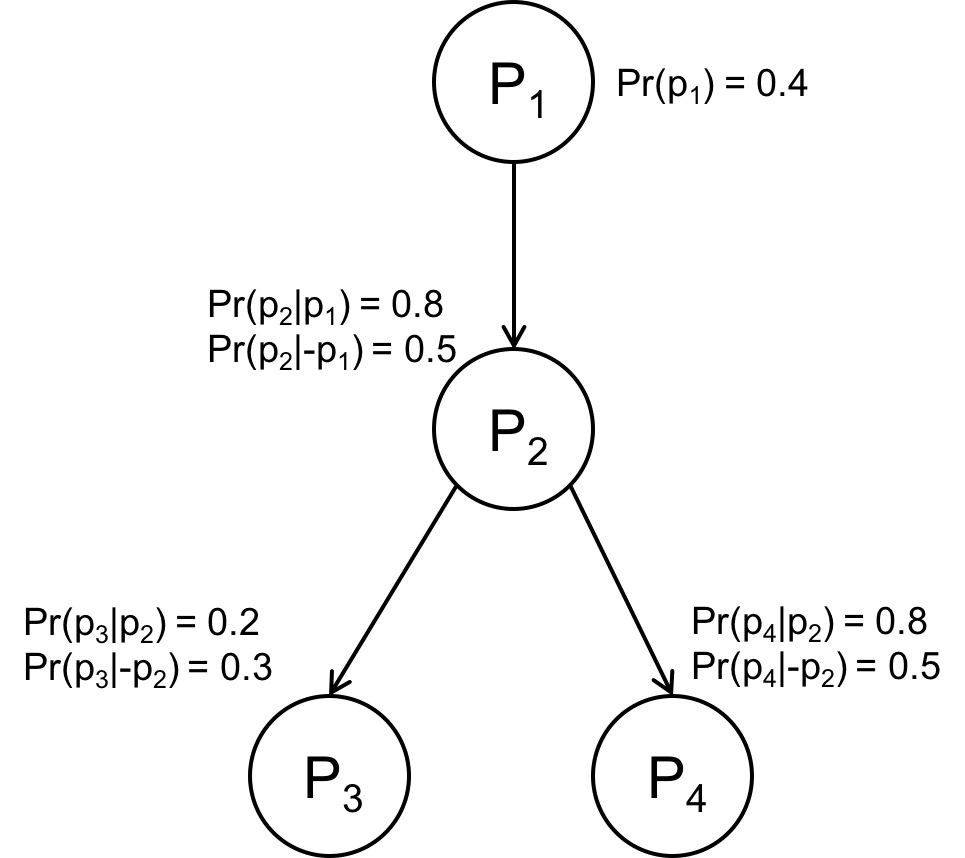
\includegraphics[width=0.6\textwidth]{bayes_leve.png}
\end{center}

\begin{enumerate}
\item Calcula $\Pr(p_1|-p_3, p_4)$ con el método de eliminación de variable.
\item Calcula aproximadamente $\Pr(p_1|p_2, -p_3)$ con el métdo de
  muestreo con pesos de verosimilitud. Genera al menos unas 20
  muestras y compara el resultado con lo obtenido por inferencia
  exacta.
\end{enumerate}

\newpage
\section{Independencia condicional en redes bayesianas}

A partir de la siguiente gráfica circula las aseveraciones correctas
\begin{center}
  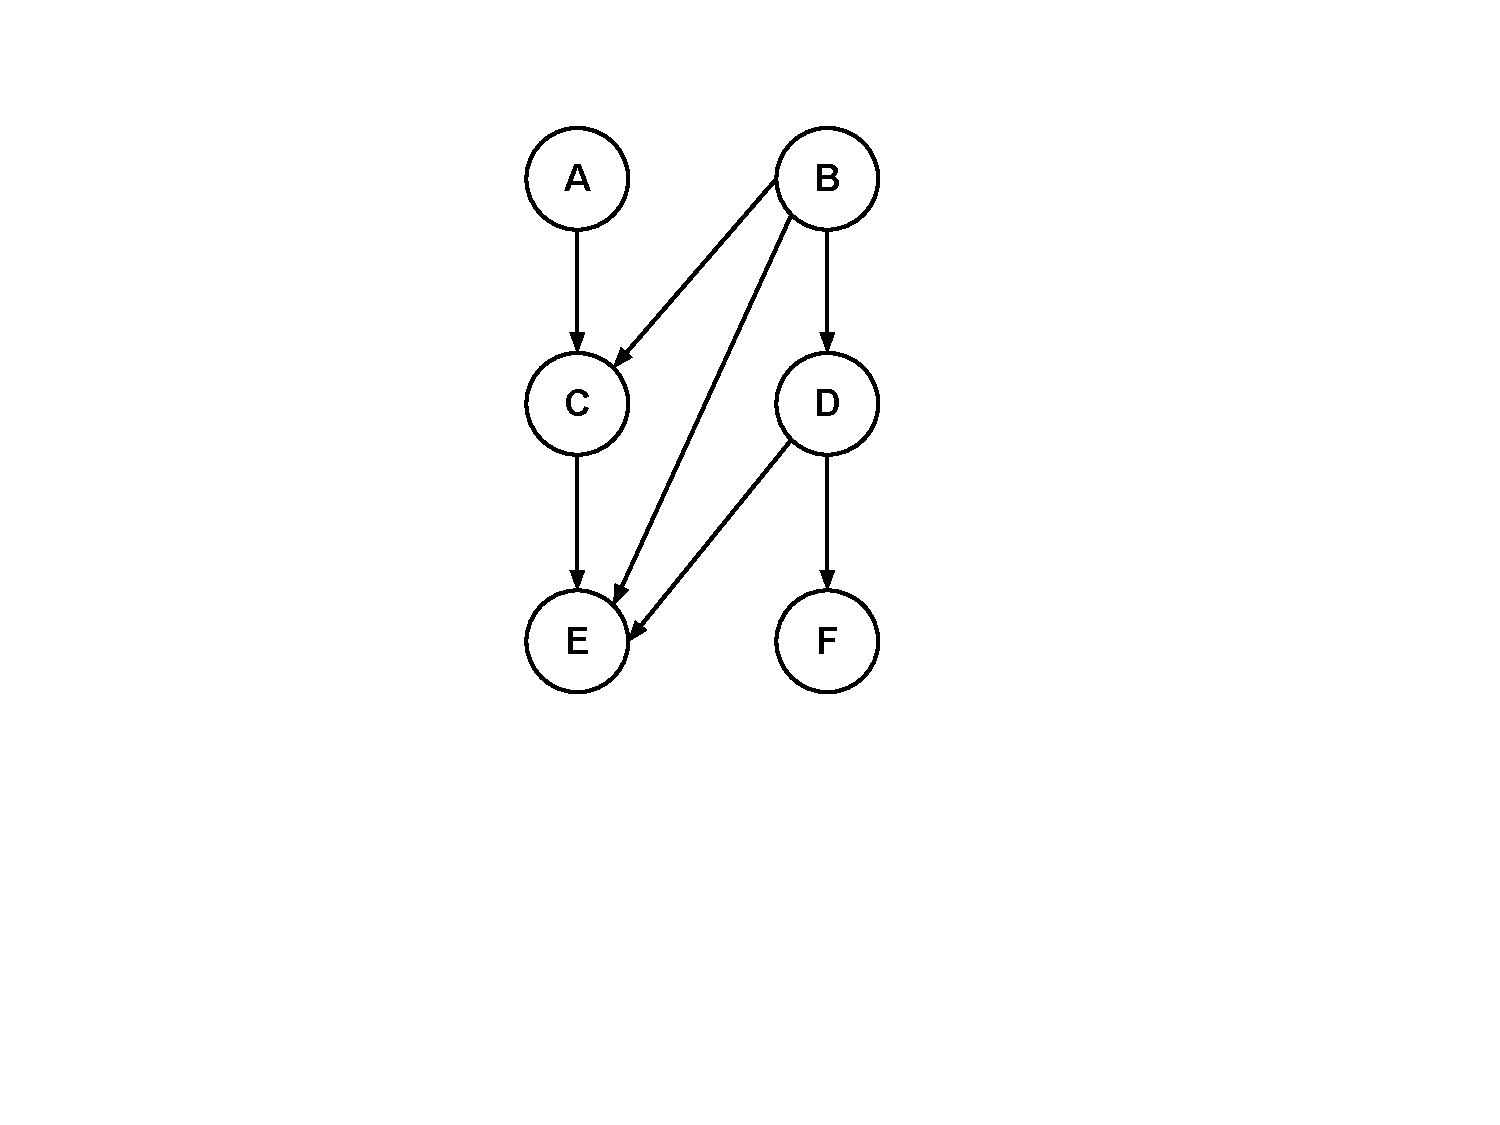
\includegraphics[width=0.3\textwidth]{red.pdf}
\end{center}

\begin{itemize}
\item $A$ es condicionalmente independiente de $C$ conociendo $D$
\item $D$ es independiente de $A$
\item $D$ es condicionalmente independiente de $A$ conociendo $E$
\item $C$ es independiente de $F$
\item $C$ es condicionalmente independiente de $F$ conociendo $B$
\item $C$ es condicionalmente independiente de $F$ conociendo $E$
\item $C$ es condicionalmente independiente de $F$ conociendo $B$ y $E$
\end{itemize}

Por último, si las variables $A$, $C$, $F$ son binarias, las variables $B$ y $E$ tienen trés valores y la variables $D$ tiene cuatro. ¿Cual es el número mínimo de parámetros que se tiene que encontrar para especificar completamente esta red bayesiana?



\end{document}
